\documentclass[12pt, a4paper]{report}
\usepackage[spanish, es-lcroman, es-noshorthands]{babel} %es-lcroman sirve para la numeración en números romanos
\usepackage[latin1, utf8]{inputenc} % podés escribir con tildes directamente
\usepackage{lmodern}
\usepackage{amsmath, amsthm, amssymb}
\usepackage{geometry}
\usepackage{enumerate}
\usepackage{graphicx}
\usepackage{amsmath}
\usepackage{amsfonts}
\usepackage{hyperref}
\usepackage{mathrsfs}
\usepackage{caption}
\usepackage{pgfplots}
\usepackage{natbib} % para la bibliografía
\usepackage[intoc, spanish]{nomencl}\makenomenclature
\setcitestyle{authoryear,open={(},close={)}}

\usepackage{listofitems} % for \readlist to create arrays
\usetikzlibrary{arrows.meta} % for arrow size
\usepackage[outline]{contour} % glow around text
\contourlength{1.4pt}

\pgfplotsset{compat = newest}
\DeclareMathAlphabet\mathrsfso{U}{rsfso}{m}{n} % para escribir letras en otras fuentes

% PARA AÑADIR CÓDIGO
% Si tu documento no tiene código de ningún tipo podés eliminar esta parte.
\usepackage{listings}
\usepackage{color}

\definecolor{dkgreen}{rgb}{0,0.6,0}
\definecolor{gray}{rgb}{0.5,0.5,0.5}
\definecolor{mauve}{rgb}{0.58,0,0.82}

\lstset{frame=tb,
  language=python,
  aboveskip=3mm,
  belowskip=3mm,
  showstringspaces=false,
  columns=flexible,
  basicstyle={\small\ttfamily},
  numbers=none,
  numberstyle=\tiny\color{gray},
  keywordstyle=\color{blue},
  commentstyle=\color{dkgreen},
  stringstyle=\color{mauve},
  breaklines=true,
  breakatwhitespace=true,
  tabsize=3
}

% OCULTAR EN EL TOC
% Lo utilizo para ocultar la aparición de \chapter{blablabla} en el toc
% para los capítulos de apéndices y anexos
\newcounter{oldtocdepth}
\newcommand{\hidefromtoc}{%
  \setcounter{oldtocdepth}{\value{tocdepth}}%
  \addtocontents{toc}{\protect\setcounter{tocdepth}{-10}}%
}
\newcommand{\unhidefromtoc}{%
  \addtocontents{toc}{\protect\setcounter{tocdepth}{\value{oldtocdepth}}}%
}
\usepackage{hyperref}
\usepackage{bookmark}

% CONFIGURAR LA NOMENCLATURA
\renewcommand{\nomgroup}[1]{%
\ifthenelse{\equal{#1}{A}}{\item[\textbf{Símbolos Romanos}]}{%
\ifthenelse{\equal{#1}{G}}{\item[\textbf{Símbolos Griegos}]}{%
\ifthenelse{\equal{#1}{Z}}{\item[\textbf{Acrónimos / Abreviaciones}]}{%
\ifthenelse{\equal{#1}{R}}{\item[\textbf{Superíndices}]}{%
\ifthenelse{\equal{#1}{S}}{\item[\textbf{Subíndices}]}{%
\ifthenelse{\equal{#1}{X}}{\item[\textbf{Otros Símbolos}]}
{}
}% matches mathematical symbols > X
}% matches Subscripts           > S
}% matches Superscripts         > R
}% matches Abbreviations        > Z
}% matches Greek Symbols        > G
}% matches Roman Symbols        > A

% PARAMETROS PARA LAS GRAFICAS DE LAS REDES NEURONALES
% En caso que no las necesites puedes borrar esta parte
%\tikzset{>=latex} % for LaTeX arrow head
\usepackage{xcolor}
\colorlet{myred}{red!80!black}
\colorlet{myblue}{blue!80!black}
\colorlet{mygreen}{green!60!black}
\colorlet{myorange}{orange!70!red!60!black}
\colorlet{mydarkred}{red!30!black}
\colorlet{mydarkblue}{blue!40!black}
\colorlet{mydarkgreen}{green!30!black}
\tikzstyle{node}=[thick,circle,draw=myblue,minimum size=22,inner sep=0.5,outer sep=0.6]
\tikzstyle{node in}=[node,green!20!black,draw=mygreen!30!black,fill=mygreen!25]
\tikzstyle{node hidden}=[node,blue!20!black,draw=myblue!30!black,fill=myblue!20]
\tikzstyle{node convol}=[node,orange!20!black,draw=myorange!30!black,fill=myorange!20]
\tikzstyle{node out}=[node,red!20!black,draw=myred!30!black,fill=myred!20]
\tikzstyle{connect}=[thick,mydarkblue] %,line cap=round
\tikzstyle{connect arrow}=[-{Latex[length=4,width=3.5]},thick,mydarkblue,shorten <=0.5,shorten >=1]
\tikzset{ % node styles, numbered for easy mapping with \nstyle
  node 1/.style={node in},
  node 2/.style={node hidden},
  node 3/.style={node out},
}
\def\nstyle{int(\lay<\Nnodlen?min(2,\lay):3)} % map layer number onto 1, 2, or 3

% BIBLIOGRAFIA
\newlength\mybibindent
\setlength\mybibindent{0pt}
\makeatletter
\renewenvironment{thebibliography}[1]
    {\chapter*{\bibname}%
     \@mkboth{\MakeUppercase\bibname}{\MakeUppercase\bibname}%
     \list{\@biblabel{\@arabic\c@enumiv}}
          {\settowidth\labelwidth{\@biblabel{999}}
           \leftmargin\labelwidth
            \advance\leftmargin\dimexpr\labelsep+\mybibindent\relax\itemindent-\mybibindent
           \@openbib@code
           \usecounter{enumiv}
           \let\p@enumiv\@empty
           \renewcommand\theenumiv{\@arabic\c@enumiv}}
     \sloppy
     \clubpenalty4000
     \@clubpenalty \clubpenalty
     \widowpenalty4000%
     \sfcode`\.\@m}
    {\def\@noitemerr
      {\@latex@warning{Empty `thebibliography' environment}}
     \endlist}
\makeatother



% MARGENES DE TEXTO
\geometry{twoside, 
  paperheight = 24.0cm,
  paperwidth = 17.0cm,
  columnsep = 1.0cm,
  textheight = 19.0cm,
  textwidth = 12.8cm,
  centering,
  marginparwidth = 1cm,
  top = 3.0cm}

% ESPACIADO Y PENALTIES  
\parskip=0.5pt plus 1.0pt minus 0.5pt
\addtolength{\skip\footins}{1pt plus 5pt minus 1pt}

\clubpenalty=225
\widowpenalty=225
\displaywidowpenalty=75

% ESTILOS TEOREMA
% Si querés cambiar la numeración podés cambiar el texto entre corchetes
\newtheorem{ejercicio}{Ejercicio}[chapter]
\newtheorem{ejemplo}{Ejemplo}[chapter]
\newtheorem{obs}{Observación}[chapter]
\newtheorem{teorema}{Teorema}[chapter]
\newtheorem{lema}{Lema}[chapter]
\newtheorem{corolario}{Corolario}[chapter]
\newtheorem{defi}{Definición}[chapter]
\newtheorem{propos}{Proposición}[chapter]

\makeatletter
% TÍTULO, AUTOR Y AÑO DE PUBLICACIÓN
% En esta parte se puede editar el texto entre llaves.
\title{Título espectacular para tu tesis}\let\Title\@title
\author{Rodrigo Pari}        \let\Author\@author
\date{2022}                         \let\Date\@date

% DEFINIENDO NUEVOS MACROS
% En esta parte se definen los macros de los comandos que usaré para la portada, no se debe editar.
\newcommand{\@universidad}{}
\newcommand{\universidad}[1]{\renewcommand{\@universidad}{#1}}

\newcommand{\@facultad}{}
\newcommand{\facultad}[1]{\renewcommand{\@facultad}{#1}}

\newcommand{\@carrera}{}
\newcommand{\carrera}[1]{\renewcommand{\@carrera}{#1}}

\newcommand{\@tutor}{}
\newcommand{\tutor}[1]{\renewcommand{\@tutor}{#1}}

\newcommand{\@departamento}{}
\newcommand{\departamento}[1]{\renewcommand{\@departamento}{#1}}

\newcommand{\@pais}{}
\newcommand{\pais}[1]{\renewcommand{\@pais}{#1}}

% INFORMACIÓN ADICIONAL
% En esta parte sí se puede editar el texto entre llaves.

% Universidad
\universidad{UNIVERSIDAD MAYOR DE SAN ANDRÉS}\let\Universidad\@universidad
% Facultad
\facultad{FACULTAD DE CIENCIAS PURAS Y NATURALES}\let\Facultad\@facultad
% Carrera
\carrera{CARRERA DE MATEMÁTICAS}\let\Carrera\@carrera
% Tutor
\tutor{Dr. Latex}\let\Tutor\@tutor
% Departamento
\departamento{La Paz}\let\Departamento\@departamento
% País
\pais{Bolivia}\let\Pais\@pais

\makeatother

% CAMBIAR TEXTO EN ÍNDICES
% Esta parte cambia el nombre con el que tendremos nuestras listas en la
% tabla de contenidos
\renewcaptionname{spanish}{\contentsname}{Tabla de contenidos}
\renewcaptionname{spanish}{\listfigurename}{Lista de figuras}
\renewcaptionname{spanish}{\listtablename}{Lista de tablas}

\begin{document}
% TEXTO PREVIO
% Las primeras páginas suelen numerarse con números romanos en minúscula.
\pagenumbering{roman}

    %\fontfamily{cmr}
\begin{titlepage}
    \begin{center}
        \textbf{\Universidad}
        
        \textbf{\Facultad}
        
        \textbf{\Carrera}
        
        \vspace{1cm}
        
         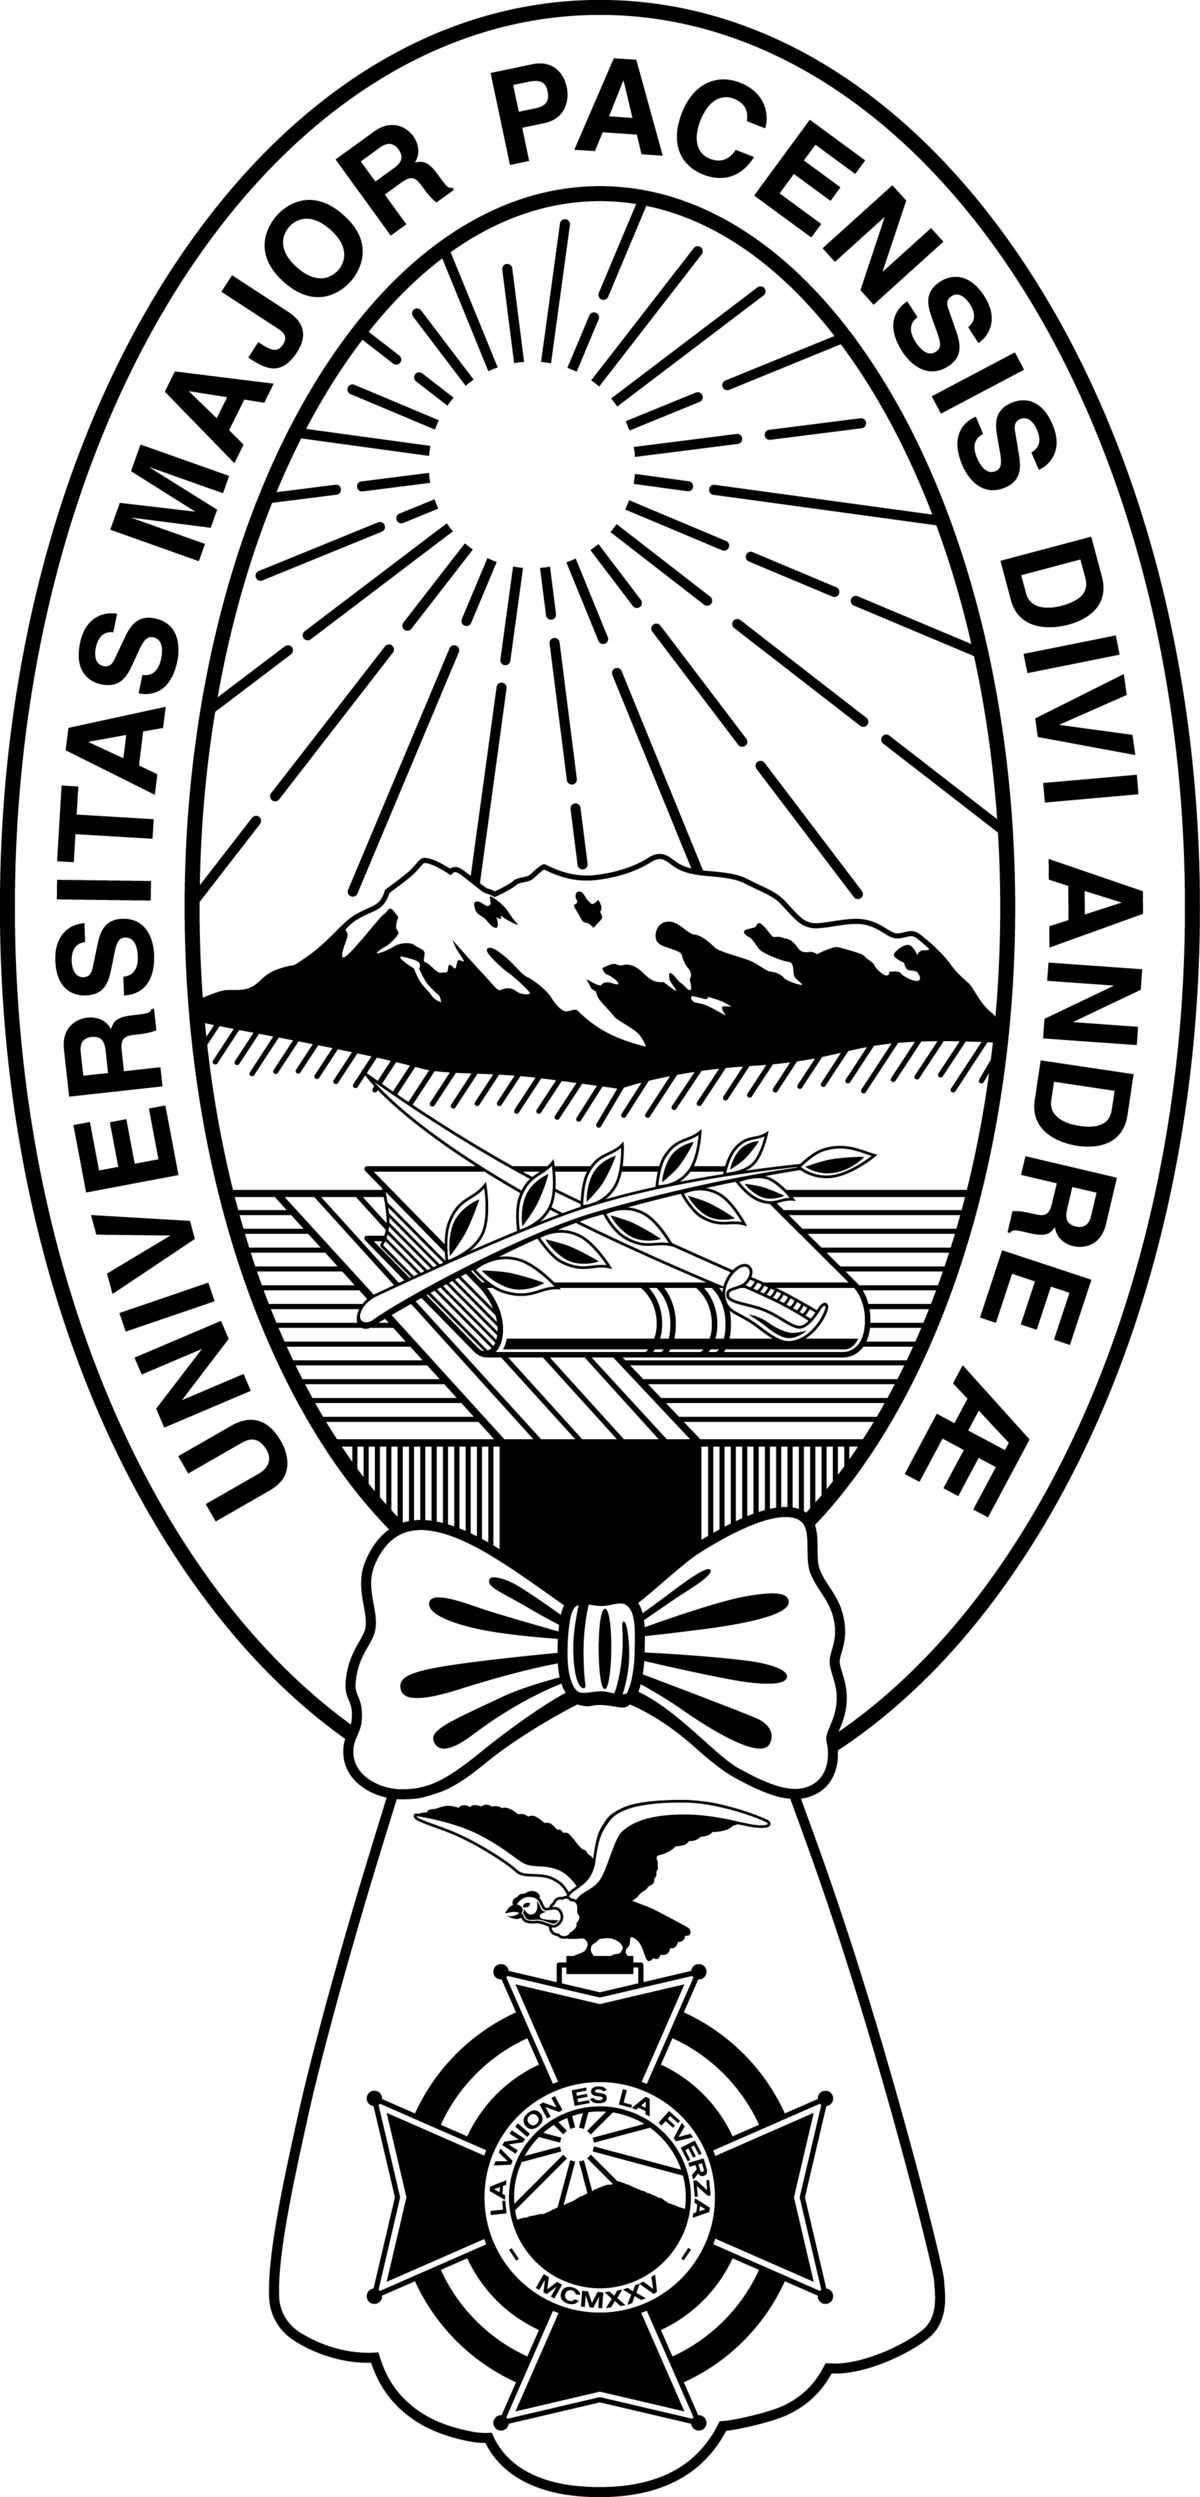
\includegraphics[width=2.9cm, height=6cm]{Imagenes/Logo UMSA.png}
         
         \vspace{1cm}
        
        
        {\Large\textbf{\Title}}\\
        
         \vspace{1cm}
         
         \textbf{POR}\\

        \vspace{1cm}
        
        \begin{tabular}{l l}
             POSTULANTE:&  \Author\\
             TUTOR:& \Tutor
        \end{tabular}
        
        \end{center}
        
        \vspace{1cm}
        \begin{center}
        \textbf{como requisito parcial para obtener el grado de\\
        Licenciado en Matemáticas}
        \end{center}

        \vspace{1cm}
        
        \begin{center}
        \textbf{\Departamento, \Pais}
        
        \textbf{\Date}
        \end{center}
    
\end{titlepage}
    % En las tesis de la UMSA no se suelen incluir las páginas de Comite
    % de Tesis o Asesor Externo, tampoco tengo datos claros sobre si la
    % universidad paga derechos de autor para las tesis de grado.
    
    %\begin{titlepage}
    
    \begin{center}
    \textbf{Título}\\
    
    \vspace{0.8cm}
    
        \textbf{Comité de Tesis}
        
          \vspace{0.7cm}
        
         $\underset{\text{\normalsize Nombre del presidente}}{\underline{\hspace{8cm}}}$\\
         \vspace{0.2cm}
         \textrm{Presidente}
         
        \vspace{0.7cm}
         
         $\underset{\text{\normalsize Nombre del secretario}}{\underline{\hspace{8cm}}}$\\
         \vspace{0.2cm}
         \textrm{Secretario}
         
         \vspace{0.7cm}
         
        $\underset{\text{\normalsize Nombre del vocal 1}}{\underline{\hspace{8cm}}}$\\
         \vspace{0.2cm}
         \textrm{Vocal}
         
         \vspace{0.7cm}
         
         $\underset{\text{\normalsize Nombre del vocal 2}}{\underline{\hspace{8cm}}}$\\
         \vspace{0.2cm}
         \textrm{Vocal}
         
         \vspace{0.7cm}
         
         $\underset{\text{\normalsize Nombre del vocal 3}}{\underline{\hspace{8cm}}}$\\
         \vspace{0.2cm}
         \textrm{Vocal}
         
         \vspace{0.7cm}
        
         $\underset{\text{\normalsize Nombre del Subdirector de Posgrado}}{\underline{\hspace{8cm}}}$\\
         \vspace{0.2cm}
         \textrm{Subdirector de Posgrado}
        
    \end{center}
\end{titlepage}
    
    %\begin{titlepage}
    
    \begin{center}
    \textbf{Titulo}\\
    
    \vspace{1cm}
    
        \textbf{Dirección de Tesis}
        
          \vspace{1.5cm}
        
         $\underset{\text{\normalsize Nombre del director}}{\underline{\hspace{8cm}}}$\\
         \vspace{0.2cm}
         \textrm{Director}
         
        \vspace{1.5cm}
         
         $\underset{\text{\normalsize Nombre del asesor externo}}{\underline{\hspace{8cm}}}$\\
         \vspace{0.2cm}
         \textrm{Asesor Externo}
        
    \end{center}
\end{titlepage}
    
    \thispagestyle{empty}
\begin{center}
Dedico esto a...
\end{center}

\newpage
    \thispagestyle{empty}
\vspace*{\fill}
\begin{center}
Copyright \copyright  \thinspace 2022 por Rodrigo Pari Susaño \\ Todos Los Derechos Reservados
\end{center}
\vspace*{\fill}

\newpage
    \chapter*{\centering \Large Agradecimientos}

Quiero agradecer a...
    \chapter*{\centering \Large Declaración}


Por la presente declaro que, este documento es una compilación de trabajos previos, disertaciones, papers y textos académicos tal y como se especifica en las referencias y agradecimientos. Salvo que se señale lo contrario, los resultados que se hallan en el documento no son de mi autoría. Esta compilación es original y no se ha presentado para su consideración para ningún otro título o calificación en esta u otra universidad. Esta disertación contiene menos de 65,000 palabras incluyendo apéndices, anexos, bibliografía, notas al pie, tablas y ecuaciones y tiene menos de 150 figuras.

{\flushright
\Author\\
\Date
\vfill}
% El autor y la fecha se añadirán automáticamente desde info.tex 
    
    \chapter*{\centering \Large Resumen}

Este trabajo trata de...
    
    % Solo la lista de figuras, tablas y nomenclatura aparecerán en la
    % tabla de contenidos.

    % Si no aparece la nomenclatura (puede pasar si no lo compilás
    % overleaf),  en cmd hacé lo siguiente
    % usando cd entra a la carpeta en la que esta tu proyecto
    % por ejemplo, si esta en el disco C, en la dirección, User\tesis
    % se vería así
    % cd C:\User\tesis
    % ahora, suponiendo que este archivo tenga el nombre main.tex
    % escribí lo siguiente en cmd y apretá enter.
    % makeindex main.nlo -s nomencl.ist -o main.nls
    % suponiendo que este archivo se llame main.tex
    
    \cleardoublepage\tableofcontents\setcounter{tocdepth}{2}
    \cleardoublepage\listoffigures \addcontentsline{toc}{chapter}{Lista de figuras}\setcounter{tocdepth}{2}
    \cleardoublepage\listoftables \addcontentsline{toc}{chapter}{Lista de tablas}\setcounter{tocdepth}{2}
    \cleardoublepage\printnomenclature
    
    \newpage

% CAPÍTULOS    
\pagenumbering{arabic}
    
    \chapter{Introducción}
    Este documento tratará varias cosas y se explicará cada una de ellas.

\begin{itemize}
    \item En el capítulo 1 introduciremos.
    \item En el capítulo 3 concluiremos.
\end{itemize}

Podemos citar los siguientes autores \cite{ash}, \cite{brezis}
    
    \chapter{Redes neuronales prealimentadas}
    Una red neuronal prealimentada (a partir de ahora FNN), es un modelo compuesto por \textit{capas}.

\newpage

\begin{figure}[h!]
    \centering
    \begin{tikzpicture}[x=2.2cm,y=1.4cm]
        \readlist\Nnod{3,4,4,4,3} % array of number of nodes per layer
        \readlist\Nstr{n,m,m,m,k} % array of string number of nodes per layer
        \readlist\Cstr{\strut x,a^{(\prev)},a^{(\prev)},a^{(\prev)},y} % array of coefficient symbol per layer
        \def\yshift{0.5} % shift last node for dots
        
        \message{^^J  Layer}
        \foreachitem \N \in \Nnod{ % loop over layers
        \def\lay{\Ncnt} % alias of index of current layer
        \pgfmathsetmacro\prev{int(\Ncnt-1)} % number of previous layer
        \message{\lay,}
        \foreach \i [evaluate={\c=int(\i==\N); \y=\N/2-\i-\c*\yshift;
                     \index=(\i<\N?int(\i):"\Nstr[\lay]");
                     \x=\lay; \n=\nstyle;}] in {1,...,\N}{ % loop over nodes
          % NODES
          \node[node \n] (N\lay-\i) at (\x,\y) {$\Cstr[\lay]_{\index}$};
          
          % CONNECTIONS
          \ifnum\lay>1 % connect to previous layer
            \foreach \j in {1,...,\Nnod[\prev]}{ % loop over nodes in previous layer
              \draw[connect,white,line width=1.2] (N\prev-\j) -- (N\lay-\i);
              \draw[connect] (N\prev-\j) -- (N\lay-\i);
              %\draw[connect] (N\prev-\j.0) -- (N\lay-\i.180); % connect to left
            }
          \fi % else: nothing to connect first layer
          
        }
        \path (N\lay-\N) --++ (0,1+\yshift) node[midway,scale=1.5] {$\vdots$};
        }
        
        % LABELS
        \node[above=5,align=center,mygreen!60!black] at (N1-1.90) {capa de\\[-0.2em]entrada};
        %\node[above=2,align=center,myblue!60!black] at (N3-1.90) {capas ocultas};
        \node[above=2,align=center,myblue!60!black] at (N3-1.90) {capas ocultas};
        \node[above=10,align=center,myred!60!black] at (N\Nnodlen-1.90) {capa de\\[-0.2em]salida};
        
    \end{tikzpicture}
    \caption{Red neuronal gigante.}
    \label{fig:fnn1}
\end{figure}

Observe también que podemos añadir la siguiente tabla.

\begin{table}[h!]
    \centering
    \begin{tabular}{||c c c c||} 
     \hline
     Col1 & Col2 & Col2 & Col3 \\ [0.5ex] 
     \hline\hline
     1 & 6 & 87837 & 787 \\ 
     2 & 7 & 78 & 5415 \\
     3 & 545 & 778 & 7507 \\
     4 & 545 & 18744 & 7560 \\
     5 & 88 & 788 & 6344 \\ [1ex] 
     \hline
    \end{tabular}
    \caption{Tabla con valores sin sentido.}
    \label{table:1}
    \end{table}

Ahora algunas ecuaciones.

\begin{defi}
La función \textit{rectificadora} se define como

\begin{align*}
    ReLU \colon \mathbb{R} &\to \mathbb{R}\\
    x &\mapsto max\{0, x\}
\end{align*}

\begin{figure}[h!]
    \centering
    \begin{tikzpicture}
        \begin{axis}
            domain=-4:4,
            ]
            \addplot+[mark=none,red,domain=-4:0] {0};
            \addplot+[mark=none,red,domain=0:4] {x};
        \end{axis}
    \end{tikzpicture}
    \caption{Gráfico de la función ReLU}
    \label{fig:relu}
\end{figure}

\end{defi}

\newpage

\section{Función sigmoidea}

\begin{obs}
Una función sigmoidea muy conocída es la \textit{sigmoide}

\newpage

\begin{align*}
    \sigma \colon \mathbb{R} &\to \mathbb{R}\\
    x &\mapsto \frac{1}{1 + e^{-x}}
\end{align*}

\begin{figure}[h!]
    \centering
    \begin{tikzpicture}
        \begin{axis}
            domain=-4:4,
            ]
            \addplot[red,mark=none,domain=-4:4]   (x,{1/(1+exp(-\x))});
        \end{axis}
    \end{tikzpicture}
    \caption{Gráfico de la función sigmoide}
    \label{fig:sigmoide}
\end{figure}
\end{obs}


    
    \chapter{Conclusión}
    Concluímos que esta es una plantilla para tesis.

% NOMENCLATURA
% El siguiente espacio contiene los términos que aparecerán en la página
% nomenclatura.
\nomenclature[z-FNN]{FNN}{Red Neuronal Prealimenrada (Feedforward Neural Network)}
\nomenclature[z-DNN]{DNN}{Red Neuronal Profunda (Deep Neural Network)}
\nomenclature[z-CMAT]{CMAT}{Carrera de matemáticas.}
\nomenclature[a-L]{L}{Conjunto de funciones integrables.}
\nomenclature[g-theta]{$\theta$}{Ángulo.}
\nomenclature[r-c]{$c$}{Complemento de un conjunto.}
\nomenclature[s-i]{$i$}{Valor inicial, por ejemplo, en una ecuación diferencial.}
\nomenclature[x-R]{$\mathbb{R}$}{Números reales.}

% BILIOGRAFÍA
% La referencia se añade directamente de los autores que citaste en el
% archivo references.bib
\renewcommand\bibname{Referencias}
\bibliography{references}
\addcontentsline{toc}{chapter}{Referencias}
\bibliographystyle{apalike2}
%\bibliographystyle{plain}

% SECCIONES FINALES
% Anexos y Apéndices
% Luego de pensar en varias formas de numerar estas secciones en la tabla
% de contenidos, creo que la mejor manera es simplemente numerando a mano y
% eliminando el encabezado del título.

% Apéndices
\appendix
\renewcommand\appendixname{Apéndice} % cambia el texto en el encabezado

\hidefromtoc\chapter{Apéndice de ejemplo}\unhidefromtoc
\addcontentsline{toc}{chapter}{Apéndice A: Apéndice de ejemplo}
Recordá que un apéndice es un documento creado por el autor y tiene alguna utilidad en su trabajo. Los anexos son documentos externos que el autor no creó. Si creás un cuestionario, deberías ponerlo en los apéndices. Si pillás una entrevista que hizo algún periódico, esto es un anexo.

\hidefromtoc\chapter{Otro apéndice de ejemplo}\unhidefromtoc
\addcontentsline{toc}{chapter}{Apéndice B: Otro apéndice de ejemplo}
Este es un apéndice y debería entrar algo que creó el autor. El siguiente es un código en python que muestra una suma.\\

\begin{lstlisting}
# Hola python
import math

A = 6
B = A + math.pi
print(B)
\end{lstlisting}

% Anexos
\renewcommand\appendixname{Anexo} % cambia el texto en el encabezado
%\setcounter{chapter}{0} % reiniciamos el contador de capítulos

\hidefromtoc\chapter{Anexo de ejemplo}\unhidefromtoc
\addcontentsline{toc}{chapter}{Anexo C: Anexo de ejemplo}
Un anexo contiene material del cual no sos autor.

\hidefromtoc\chapter{Otro anexo de ejemplo}\unhidefromtoc
\addcontentsline{toc}{chapter}{Anexo D: Otro anexo de ejemplo}
Mira el siguiente gráfico.

\begin{figure}[h!]
    \centering
	\begin{tikzpicture}
	\begin{axis}[
	    title=Superficie regular,
	    hide axis,
	    colormap/cool,
	]
	\addplot3[
	    mesh,
	    samples=50,
	    domain=-8:8,
	]
	{sin(deg(sqrt(x^2+y^2)))/sqrt(x^2+y^2)};
	\addlegendentry{\(\frac{sin(r)}{r}\)}
	\end{axis}
	\end{tikzpicture}
    \caption{Gráfico de superficie usando tikz}
    \label{fig:scientif}
\end{figure}


\end{document}
